\documentclass[10pt,journal,a4paper]{IEEEtran}
\usepackage{tikz}
\usepackage{caption}

\begin{document}
%
% paper title
% can use linebreaks \\ within to get better formatting as desired
\title{Report for the NOOC project}
\author{Ismail Bouanani and Jean-Baptiste Cordonnier}
%
% 
%\author{}

\IEEEcompsoctitleabstractindextext{
\begin{abstract}
Here goes a short abstract
\end{abstract}
}

% make the title area
\maketitle
\IEEEdisplaynotcompsoctitleabstractindextext

\section{Introduction}

The overall length of this report should be 4 pages . 


\section{Rumor spreading protocol}

The rumor spreading protocol is the simplest algorithm we can come with in order to solve the rumor spreading problem. Given a starting node $n_0$ (the source of the gossip), we keep track of a set of informed nodes $S = \{n_0\}$. At each time step of the algorithm, each informed node will select randomly (uniformly to simplify) one of his neighbor and inform him. Step after step the informed nodes set will grow until it contains all the vertex of $G$. Once a node is informed he becomes an informer and will spread the gossip at all the following time steps.


\section{Markov chains set-up}

The analysis in the paper of Guo and Sun \cite{GuoSun} compare the problem of gossip spreading to many random walks in parallel. Whenever a node $u$ pushes the information to an uninformed node $v$, one random walk stays in $u$ and another one goes to $v$. The random walk that "stays" in the same node is called $lazy$ while the other one is non-lazy (or $\overline{lazy}$). This split of random walks represents the fact that the information is now in $u$ and in $v$, $u$ will continue to spread this knowledge in the following rounds.

\begin{figure}[h]
\centering
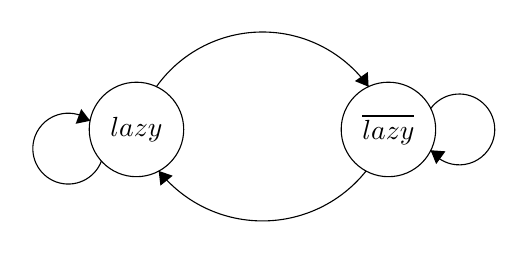
\begin{tikzpicture}[scale=0.2]
\tikzstyle{every node}+=[inner sep=0pt]
\draw [black] (26.1,-26.6) circle (3);
\draw (26.1,-26.6) node {$lazy$};
\draw [black] (42.1,-26.6) circle (3);
\draw (42.1,-26.6) node {$\overline{lazy}$};
\draw [black] (40.688,-29.229) arc (-38.4609:-141.5391:8.413);
\fill [black] (27.51,-29.23) -- (27.62,-30.17) -- (28.4,-29.54);
\draw [black] (27.358,-23.895) arc (144.65362:35.34638:8.265);
\fill [black] (40.84,-23.89) -- (40.79,-22.95) -- (39.97,-23.53);
\draw [black] (23.878,-28.598) arc (-20.31276:-308.31276:2.25);
\fill [black] (23.16,-26.05) -- (22.59,-25.3) -- (22.24,-26.24);
\draw [black] (44.78,-25.277) arc (144:-144:2.25);
\fill [black] (44.78,-27.92) -- (45.13,-28.8) -- (45.72,-27.99);
\end{tikzpicture}
\caption{Random walk state}
\label{fig:lazyFSM}
\end{figure}

We define two types of random walks when the information is spread through the graph: the forward and the backward random walks. Forward random walks start from the source $s$ while backward random walks are used only in the analysis and start from a targeted node $t$. Then to know if a node $t$ has been informed, we only need to show that there exists a node $v$ reached by a forward random walk from $s$ and a backward random walk from $t$.

We can consider all the random walks pattern after $k$ steps as $S \in \mathcal C_k = \{ lazy, \overline{lazy} \}^k$. We define the indicator random variable $X_{u,v}^S$ (resp. $Y_{u,v}^S$) that the forward (resp. backward) random walk with pattern $S$ and initial node $u$ will end up at node $v$. To show that a node $w$ is reached by the gossip in $T$ step we need to find a vertex $u$ such that $X_{s,u}^{S}Y_{w,u}^{S'} = 1$ with $|S| = |S'| = T/2$.

\section{Bound analysis}

\section{Randomness needed}

\bibliography{biblio.bib}

\end{document}


